\chapter{Bag of Words}

\newthought{Every machine learning needs numbers, but all we have is text.} A simple way to convert documents into numeric vectors is to \dots well, count the words in each text.

\begin{center}
    \begin{tabular}{c|c|c|c|c|c|c}
    Document & this & is & an & example & another & apple \\
    \hline
    \emph{This is an example} & 1 & 1 & 1 & 1 & 0 & 0 \\ 
    \emph{Another example} & 0 & 0 & 0 & 1 & 1 & 0 \\  
    \emph{This is another apple} & 1 & 1 & 0 & 0 & 1 & 1    
    \end{tabular}
\end{center}

\widget{Bag of Words} creates a table with words in columns and documents in rows. Values are word frequencies in each document.

\begin{wrapfigure}{o}{0.6\textwidth}
    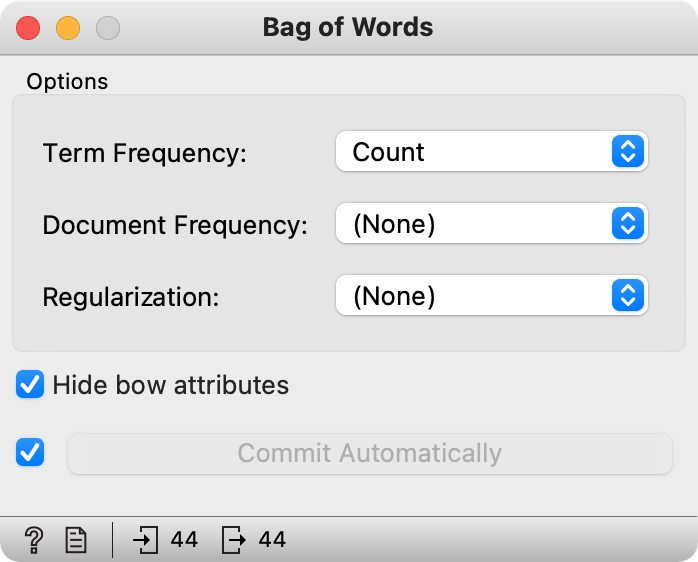
\includegraphics[scale=0.5]{bag-of-words.png}
    \caption{$\;$}
\end{wrapfigure}

We can simply count the words (TF or term frequency) or weigh the words according to how often they appear in the documents (IDF or inverse document frequency). Using TF-IDF, common words will have a low value as they appear across most documents, while significant words will have a high value because they appear frequently in a small number of documents.

Pass the data through a \widget{Bag of Words} widget and then again to a \widget{Data Table}. We get a new column that contains word counts for each document. Now that we have numbers, we can finally perform some magic!

\vspace{-0.2cm}
\begin{figure}[h]
  \centering
  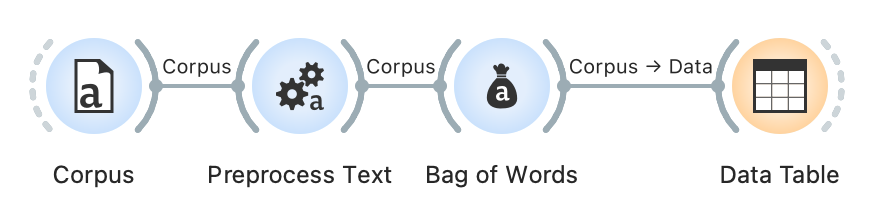
\includegraphics[width=\linewidth]{workflow.png}%
  \caption{$\;$}
\end{figure}
\vspace{-0.3cm}

\vspace{-0.2cm}
\begin{figure}[h]
  \centering
  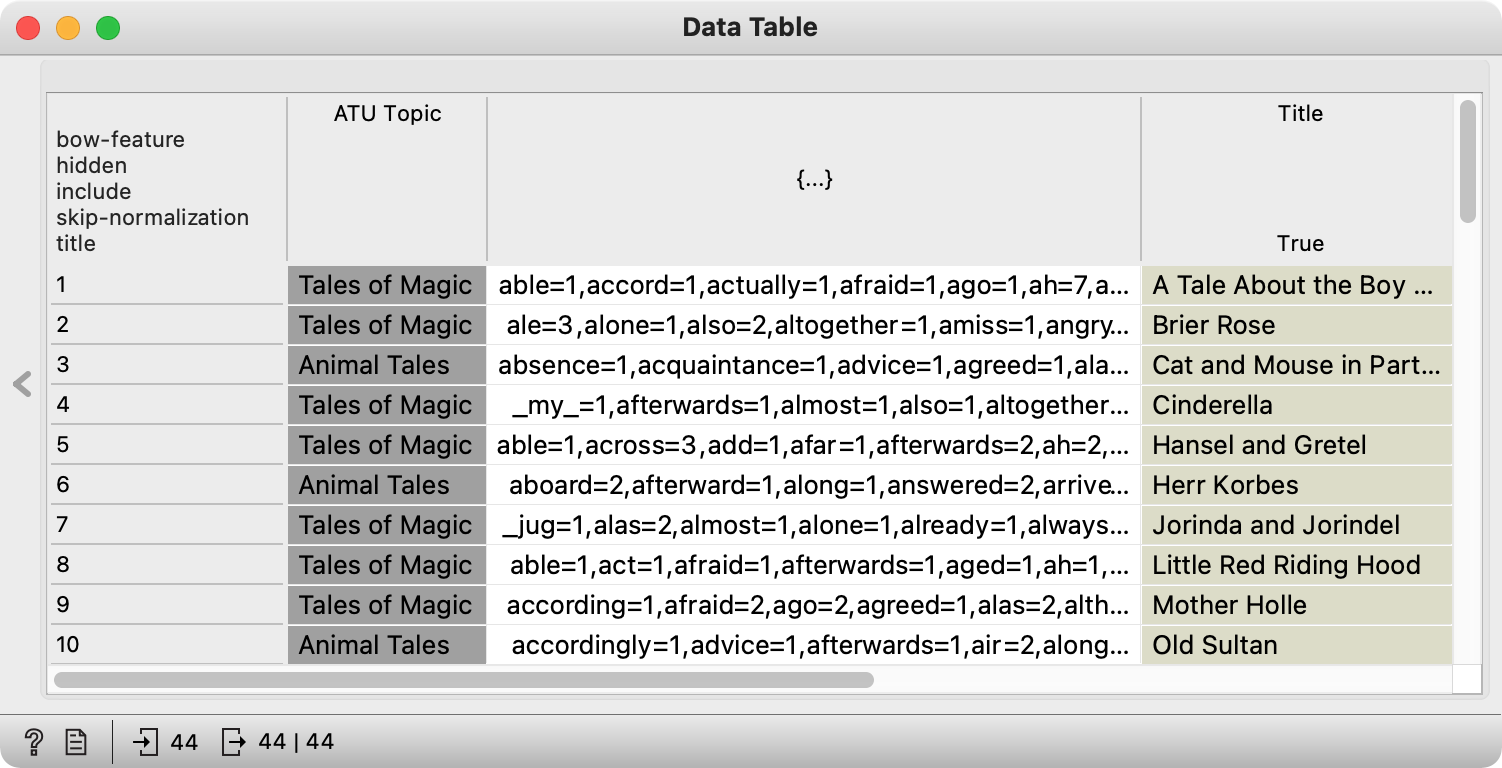
\includegraphics[width=1.2\linewidth]{data-table.png}%
  \caption{$\;$}
\end{figure}
\vspace{-0.3cm}